\documentclass[12pt]{beamer}
\usepackage{Estilos/BeamerFC}
\usepackage{Estilos/ColoresLatex}
\usetheme{Warsaw}
\usecolortheme{seahorse}
%\useoutertheme{default}
\setbeamercovered{invisible}
% or whatever (possibly just delete it)
\setbeamertemplate{section in toc}[sections numbered]
\setbeamertemplate{subsection in toc}[subsections numbered]
\setbeamertemplate{subsection in toc}{\leavevmode\leftskip=3.2em\rlap{\hskip-2em\inserttocsectionnumber.\inserttocsubsectionnumber}\inserttocsubsection\par}
\setbeamercolor{section in toc}{fg=blue}
\setbeamercolor{subsection in toc}{fg=blue}
\setbeamercolor{frametitle}{fg=blue}
\setbeamertemplate{caption}[numbered]

\setbeamertemplate{footline}
\beamertemplatenavigationsymbolsempty
\setbeamertemplate{headline}{}


\makeatletter
\setbeamercolor{section in foot}{bg=gray!30, fg=black!90!orange}
\setbeamercolor{subsection in foot}{bg=blue!30}
\setbeamercolor{date in foot}{bg=black}
\setbeamertemplate{footline}
{
  \leavevmode%
  \hbox{%
  \begin{beamercolorbox}[wd=.333333\paperwidth,ht=2.25ex,dp=1ex,center]{section in foot}%
    \usebeamerfont{section in foot} \insertsection
  \end{beamercolorbox}%
  \begin{beamercolorbox}[wd=.333333\paperwidth,ht=2.25ex,dp=1ex,center]{subsection in foot}%
    \usebeamerfont{subsection in foot}  \insertsubsection
  \end{beamercolorbox}%
  \begin{beamercolorbox}[wd=.333333\paperwidth,ht=2.25ex,dp=1ex,right]{date in head/foot}%
    \usebeamerfont{date in head/foot} {T1 - Segunda presentación} \hspace*{2em}
    \insertframenumber{} / \inserttotalframenumber \hspace*{2ex} 
  \end{beamercolorbox}}%
  \vskip0pt%
}
\makeatother

\makeatletter
\patchcmd{\beamer@sectionintoc}{\vskip1.5em}{\vskip0.8em}{}{}
\makeatother
\usepackage{pifont}
\newcommand{\cmark}{\ding{51}}%
\newcommand{\xmark}{\ding{55}}%

\makeatletter
\setbeamertemplate{footline}
{
  \leavevmode%
  \hbox{%
  \begin{beamercolorbox}[wd=.333333\paperwidth,ht=2.25ex,dp=1ex,center]{section in foot}%
    \usebeamerfont{section in foot} \insertsection
  \end{beamercolorbox}%
  \begin{beamercolorbox}[wd=.333333\paperwidth,ht=2.25ex,dp=1ex,center]{subsection in foot}%
    \usebeamerfont{subsection in foot}  \insertsubsection
  \end{beamercolorbox}%
  \begin{beamercolorbox}[wd=.333333\paperwidth,ht=2.25ex,dp=1ex,right]{date in head/foot}%
    \usebeamerfont{date in head/foot} \insertshortdate{} \hspace*{2em}
    \insertframenumber{} / \inserttotalframenumber \hspace*{2ex} 
  \end{beamercolorbox}}%
  \vskip0pt%
}
\makeatother

\setbeamertemplate{navigation symbols}{}
\date{16 de marzo}

\title{Sesión 3. Física}
\subtitle{Asesoría}

\begin{document}

\maketitle
\fontsize{14}{14}\selectfont
\spanishdecimal{.}

\section*{Contenido}
\frame[allowframebreaks]{\tableofcontents[currentsection, hideallsubsections]}

\section{Operaciones con vectores}
\frame{\tableofcontents[currentsection, hideothersubsections]}
\subsection{Suma de vectores}

\begin{frame}
\frametitle{El método del paralelogramo}
Por definición, los vectores se suman de acuerdo con la \emph{ley del paralelogramo}.
\\
\bigskip
\pause
Así, la suma de dos vectores $\va{P}$ y $\va{Q}$ se obtiene uniendo los dos vectores al mismo punto $A$ y construyendo un paralelogramo que tenga por lados a $\va{P}$ y a $\va{Q}$.
\end{frame}
\begin{frame}
\frametitle{El método del paralelogramo}
\begin{figure}
    \centering
    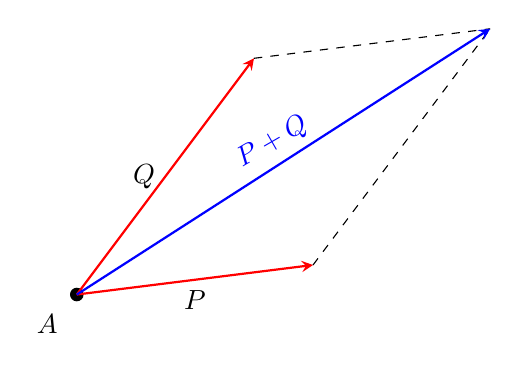
\begin{tikzpicture}[scale=1.5]
        \draw [fill] (0, 0) circle (1.5pt);
        \node at (-0.25, -0.25) {$A$};
        \draw [-stealth, thick, color=red, text=black] (0, 0) -- (2, 0.25) node [below, midway] {$\va{P}$};
        \draw [-stealth, thick, color=red, text=black] (0, 0) -- (1.5, 2) node [left, midway] {$\va{Q}$}; \pause
        \draw [dashed] (2, 0.25) -- (3.5, 2.25); \pause
        \draw [dashed] (1.5, 2) -- (3.5, 2.25); \pause
        \draw [-stealth, thick, color=blue] (0, 0) -- (3.5, 2.25) node [above, midway, rotate=30] {$\va{P} + \va{Q}$};
    \end{tikzpicture}
\end{figure}
\end{frame}
\begin{frame}
\frametitle{El vector resultante}
La diagonal que pasa por $A$ representa la suma vectorial de $\va{P}$ y $\va{Q}$, y se representa por $\va{P} + \va{Q}$.
\end{frame}
\begin{frame}
\frametitle{La regla del triángulo}
A partir de la ley del paralelogramo se puede obtener otro método para determinar
la suma de dos vectores.
\end{frame}
\begin{frame}
\frametitle{La regla del triángulo}    
Este método, llamado \textocolor{ao}{regla del triángulo}, se obtiene como sigue: \pause nos apoyamos con la siguiente figura:
\end{frame}
\begin{frame}
\frametitle{La regla del triángulo}    
\begin{figure}
    \centering
    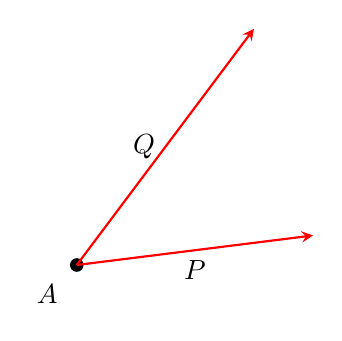
\begin{tikzpicture}[scale=1.5]
        \draw [fill] (0, 0) circle (1.5pt);
        \node at (-0.25, -0.25) {$A$};
        \draw [-stealth, thick, color=red, text=black] (0, 0) -- (2, 0.25) node [below, midway] {$\va{P}$};
        \draw [-stealth, thick, color=red, text=black] (0, 0) -- (1.5, 2) node [left, midway] {$\va{Q}$};
        % \draw [dashed] (2, 0.25) -- (3.5, 2.25); \pause
        % \draw [dashed] (1.5, 2) -- (3.5, 2.25); \pause
        % \draw [-stealth, thick, color=blue] (0, 0) -- (3.5, 2.25) node [above, midway, rotate=30] {$\va{P} + \va{Q}$};
    \end{tikzpicture}
\end{figure}
\end{frame}
\begin{frame}
\frametitle{La regla del triángulo}    
\begin{figure}
    \centering
    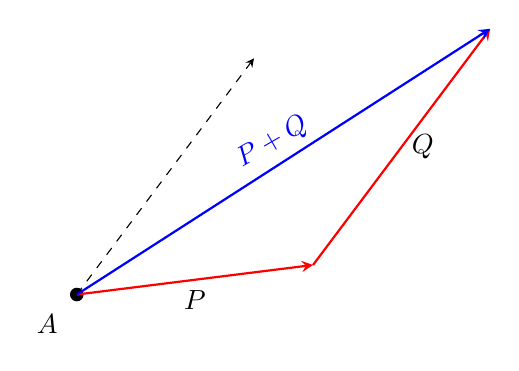
\begin{tikzpicture}[scale=1.5]
        \draw [fill] (0, 0) circle (1.5pt);
        \node at (-0.25, -0.25) {$A$};
        \draw [-stealth, thick, color=red, text=black] (0, 0) -- (2, 0.25) node [below, midway] {$\va{P}$}; \pause
        \draw [-stealth, dashed] (0, 0) -- (1.5, 2);
        \draw [-stealth, thick, color=red, text=black] (2, 0.25) -- (3.5, 2.25) node [right, midway] {$\va{Q}$}; \pause
        \draw [-stealth, thick, color=blue] (0, 0) -- (3.5, 2.25) node [above, midway, rotate=30] {$\va{P} + \va{Q}$};
    \end{tikzpicture}
\end{figure}
\end{frame}
\begin{frame}
\frametitle{La ley de triángulo}
La suma de los dos vectores puede encontrarse colocando $\va{P}$ y $\va{Q}$ de punta a cola y uniendo la cola de $\va{P}$ con la punta de $\va{Q}$.
\end{frame}
\begin{frame}
\frametitle{La regla del triángulo}    
\begin{figure}
    \centering
    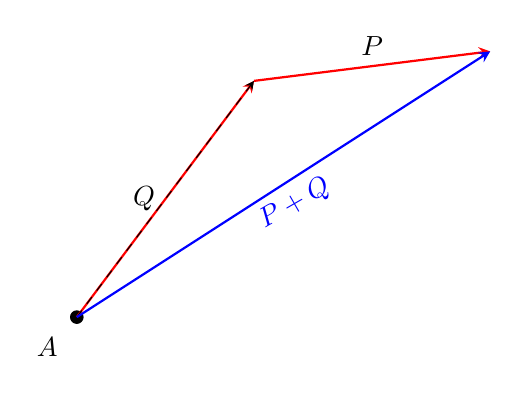
\begin{tikzpicture}[scale=1.5]
        \draw [fill] (0, 0) circle (1.5pt);
        \node at (-0.25, -0.25) {$A$};
        \draw [-stealth, thick, color=red, text=black] (0, 0) -- (1.5, 2) node [left, midway] {$\va{Q}$}; \pause
        \draw [-stealth, thick, color=red, text=black] (1.5, 2) -- (3.5, 2.25) node [above, midway] {$\va{P}$}; \pause
        \draw [-stealth, dashed] (0, 0) -- (1.5, 2);
        \draw [-stealth, thick, color=blue] (0, 0) -- (3.5, 2.25) node [below, midway, rotate=30] {$\va{P} + \va{Q}$};
    \end{tikzpicture}
\end{figure}
\end{frame}
\begin{frame}
\frametitle{La suma con más vectores}
La suma de tres vectores $\va{P}$, $\va{Q}$ y $\va{S}$ se obtiene, por definición, sumando primero los vectores $\va{P}$ y $\va{Q}$ y agregando el vector $\va{S}$ al vector $\va{P} + \va{Q}$:
\end{frame}
\begin{frame}
\frametitle{La regla del triángulo}    
\begin{figure}
    \centering
    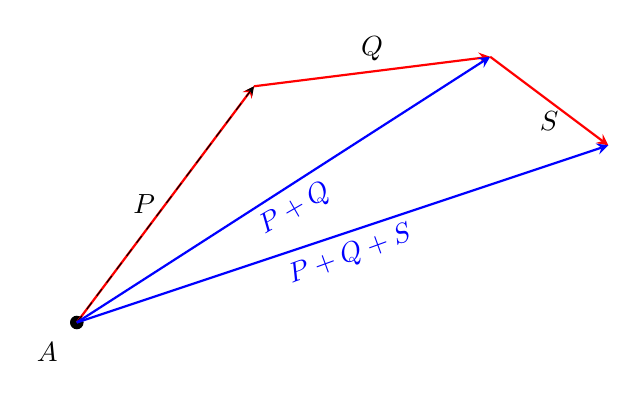
\begin{tikzpicture}[scale=1.5]
        \draw [fill] (0, 0) circle (1.5pt);
        \node at (-0.25, -0.25) {$A$};
        \draw [-stealth, thick, color=red, text=black] (0, 0) -- (1.5, 2) node [left, midway] {$\va{P}$}; \pause
        \draw [-stealth, thick, color=red, text=black] (1.5, 2) -- (3.5, 2.25) node [above, midway] {$\va{Q}$}; \pause
        \draw [-stealth, dashed] (0, 0) -- (1.5, 2);
        \draw [-stealth, thick, color=blue] (0, 0) -- (3.5, 2.25) node [below, midway, rotate=30] {$\va{P} + \va{Q}$}; \pause
        \draw [-stealth, thick, color=red, text=black] (3.5, 2.25) -- (4.5, 1.5) node [below, midway] {$\va{S}$}; \pause
        \draw [-stealth, thick, color=blue] (0, 0) -- (4.5, 1.5) node [below, midway, rotate=20] {$\va{P} + \va{Q} + \va{S}$};
    \end{tikzpicture}
\end{figure}
\end{frame}

\section{Ejercicios Guía}
\frame{\tableofcontents[currentsection, hideothersubsections]}
\subsection{Ejercicio 1}

\begin{frame}
\frametitle{Enunciado del Ejercicio 1}
En una competencia, un corredor realiza los siguientes desplazamientos:
\setbeamercolor{item projected}{bg=bananayellow,fg=blue}
\setbeamertemplate{enumerate items}{%
\usebeamercolor[bg]{item projected}%
\raisebox{1.5pt}{\colorbox{bg}{\color{fg}\footnotesize\insertenumlabel}}%
}
\begin{enumerate}[<+->]
\item $d_{1} = \SI{400}{\meter}, \theta = \ang{35}$
\item $d_{2} = \SI{700}{\meter}, \theta = \ang{120}$
\item $d_{3} = \SI{600}{\meter}, \theta = \ang{190}$
\item $d_{4} = \SI{200}{\meter}, \theta = \ang{250}$
\end{enumerate}
\end{frame}
\begin{frame}
\frametitle{Enunciado del ejercicio 1}
Encuentra gráficamente cuál es el desplazamiento resultante del corredor y cuál es el valor del ángulo del desplazamiento resultante, medido respecto al eje $x$ positivo.
\end{frame}
\begin{frame}
\frametitle{Solución al Ejercicio 1}
Utilizando el método gráfico \enquote{conectamos} los vectores con la correspondiente orientación que se indica con el ángulo de cada uno de ellos.
\end{frame}
\begin{frame}[plain]
\begin{figure}
    \centering
    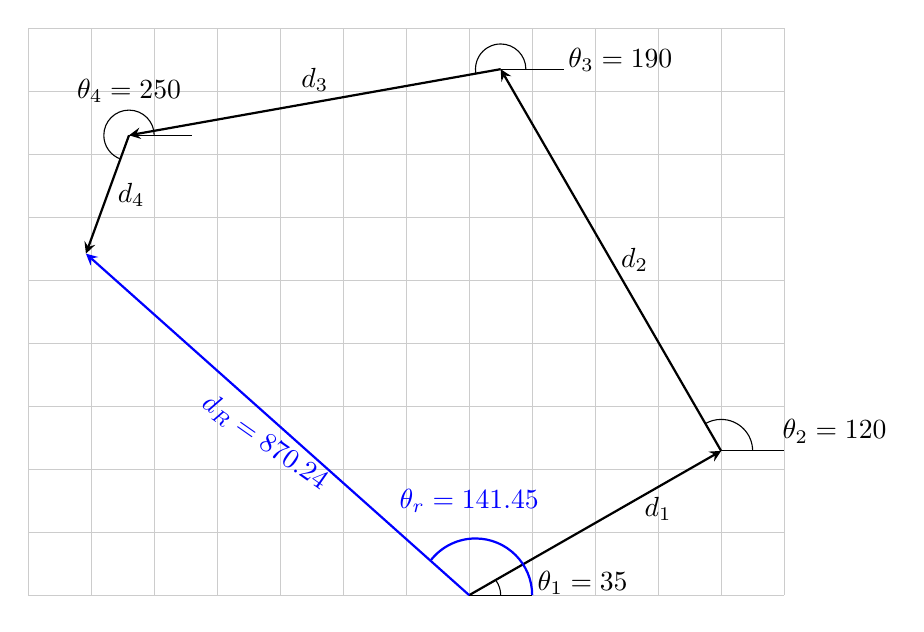
\begin{tikzpicture}[scale=0.8]
        \draw[thin, gray!40] (-7, 0) grid (5, 9);
        \draw [-stealth, thick] (0, 0) -- (4, 2.29) node [below, near end] {$d_{1}$};
        \draw (0, 0) -- (1, 0);
        \draw (0.5, 0) arc(0:35:0.4);
        \node at (1.8, 0.2) {$\theta_{1} = \ang{35}$};
        \pause
        \draw [-stealth, thick] (4, 2.29) -- (0.5, 8.35) node [midway, right] {$d_{2}$};
        \draw (4, 2.29) -- (5, 2.29);
        \draw (4.5, 2.29) arc(0:120:0.5);
        \node at (5.8, 2.6) {$\theta_{2} = \ang{120}$};
        \pause
        \draw [-stealth, thick] (0.5, 8.35) -- (-5.4, 7.3) node [above, midway] {$d_{3}$};
        \draw (0.5, 8.35) -- (1.5, 8.35);
        \draw (0.9, 8.35) arc(0:190:0.4);
        \node at (2.4, 8.5) {$\theta_{3} = \ang{190}$};
        \pause
        \draw [-stealth, thick] (-5.4, 7.3) -- (-6.084, 5.421) node [midway, right] {$d_{4}$};
        \draw (-5.4, 7.3) -- (-4.4, 7.3);
        \draw (-5, 7.3) arc(0:250:0.4);
        \node at (-5.4, 8) {$\theta_{4} = \ang{250}$};
        \pause
        \draw [-stealth, thick, color=blue] (0, 0) -- (-6.084, 5.421) node [midway, below, rotate=-35] {$d_{R} = \SI{870.24}{\meter}$}; \pause
        \draw [thick, color=blue] (1, 0) arc(0:141.45:0.9);
        \node [blue] at (0, 1.5) {$\theta_{r} = \ang{141.45}$};
    \end{tikzpicture}
\end{figure}
\end{frame}

\subsection{Método analítico}

\begin{frame}
\frametitle{Descomposición en componentes}
Es sabido que todo vector $\va{A}$ se puede \enquote{descomponer} en las llamadas \emph{componentes}, tanto en la dirección del eje $x$, como del eje $y$. 
\end{frame}
\begin{frame}
\frametitle{Base geométrica}
Para obtener las componentes del vector, recordemos de la geometría, el caso de un triángulo rectángulo: \pause
\begin{figure}
    \centering
    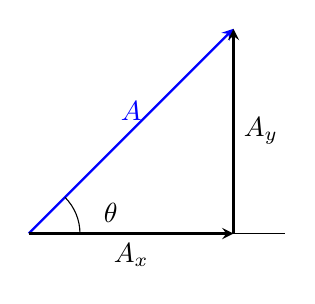
\begin{tikzpicture}[scale=1.3]
        \draw [-stealth, thick, color=blue] (0, 0) -- (2, 2) node [above, midway] {$\va{A}$};
        \draw (0.5, 0) arc(0:45:0.5);
        \node at (0.8, 0.2) {$\theta$};
        \draw (0, 0) -- (2.5, 0); \pause
        \draw [-stealth, thick] (2, 0) -- (2, 2) node [right, midway] {$A_{y}$}; \pause
        \draw [-stealth, thick] (0, 0) -- (2, 0) node [below, midway] {$A_{x}$};
    \end{tikzpicture}
\end{figure}
\end{frame}
\begin{frame}
\frametitle{Base geométrica}
\begin{figure}
    \centering
    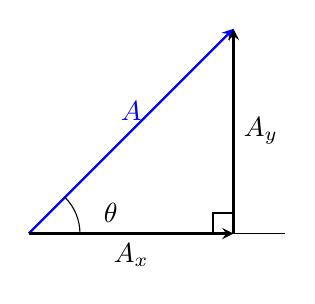
\begin{tikzpicture}[scale=1.3]
        \draw [-stealth, thick, color=blue] (0, 0) -- (2, 2) node [above, midway] {$\va{A}$};
        \draw (0.5, 0) arc(0:45:0.5);
        \node at (0.8, 0.2) {$\theta$};
        \draw (0, 0) -- (2.5, 0);
        \draw [-stealth, thick] (2, 0) -- (2, 2) node [right, midway] {$A_{y}$};
        \draw [-stealth, thick] (0, 0) -- (2, 0) node [below, midway] {$A_{x}$};
        \draw (1.8, 0) -- (1.8, 0.2) -- (2, 0.2);
    \end{tikzpicture}
\end{figure}
Las componentes del vector son:
\begin{eqnarray*}
\begin{aligned}
A_{x} &= \cos \theta \, \abs{A} \\[0.5em] \pause
A_{y} &= \sin \theta \, \abs{A}
\end{aligned}
\end{eqnarray*}
\end{frame}
\begin{frame}
\frametitle{Base geométrica}
\begin{figure}
    \centering
    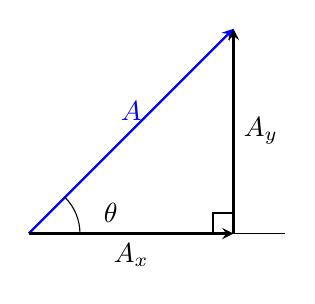
\begin{tikzpicture}[scale=1.3]
        \draw [-stealth, thick, color=blue] (0, 0) -- (2, 2) node [above, midway] {$\va{A}$};
        \draw (0.5, 0) arc(0:45:0.5);
        \node at (0.8, 0.2) {$\theta$};
        \draw (0, 0) -- (2.5, 0);
        \draw [-stealth, thick] (2, 0) -- (2, 2) node [right, midway] {$A_{y}$};
        \draw [-stealth, thick] (0, 0) -- (2, 0) node [below, midway] {$A_{x}$};
        \draw (1.8, 0) -- (1.8, 0.2) -- (2, 0.2);
    \end{tikzpicture}
\end{figure}
La magnitud del vector $\va{A}$ es:
\pause
\begin{align*}
\abs{\va{A}} = \sqrt{(A_{x})^{2} + (A_{y})^{2}}
\end{align*}
\end{frame}
\begin{frame}
\frametitle{Base geométrica}
\begin{figure}
    \centering
    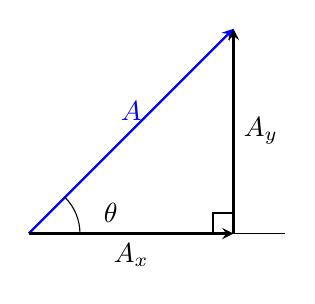
\begin{tikzpicture}[scale=1.3]
        \draw [-stealth, thick, color=blue] (0, 0) -- (2, 2) node [above, midway] {$\va{A}$};
        \draw (0.5, 0) arc(0:45:0.5);
        \node at (0.8, 0.2) {$\theta$};
        \draw (0, 0) -- (2.5, 0);
        \draw [-stealth, thick] (2, 0) -- (2, 2) node [right, midway] {$A_{y}$};
        \draw [-stealth, thick] (0, 0) -- (2, 0) node [below, midway] {$A_{x}$};
        \draw (1.8, 0) -- (1.8, 0.2) -- (2, 0.2);
    \end{tikzpicture}
\end{figure}
El valor del ángulo $\theta$ es:
\pause
\begin{align*}
\theta = \tan \left( \dfrac{A_y}{A_{x}} \right)
\end{align*}
\end{frame}

\end{document}